\documentclass{beamer}
\usepackage{listings}

\lstset{
%language=C,
frame=single, 
breaklines=true,
columns=fullflexible
}
\usepackage{subcaption}
\usepackage{url}
\usepackage{tikz}
\usepackage{tkz-euclide} % loads  TikZ and tkz-base
%\usetkzobj{all}
\usetikzlibrary{calc,math}
\usepackage{float}
\newcommand\norm[1]{\left\lVert#1\right\rVert}
\renewcommand{\vec}[1]{\mathbf{#1}}
\usepackage[export]{adjustbox}
\usepackage[utf8]{inputenc}
\usepackage{amsmath}
\usetheme{Boadilla}
\providecommand{\pr}[1]{\ensuremath{\Pr\left(#1\right)}}
\providecommand{\sbrak}[1]{\ensuremath{{}\left[#1\right]}}
\providecommand{\lsbrak}[1]{\ensuremath{{}\left[#1\right.}}
\providecommand{\rsbrak}[1]{\ensuremath{{}\left.#1\right]}}
\providecommand{\brak}[1]{\ensuremath{\left(#1\right)}}
\providecommand{\lbrak}[1]{\ensuremath{\left(#1\right.}}
\providecommand{\rbrak}[1]{\ensuremath{\left.#1\right)}}
\providecommand{\cbrak}[1]{\ensuremath{\left\{#1\right\}}}
\providecommand{\lcbrak}[1]{\ensuremath{\left\{#1\right.}}
\providecommand{\rcbrak}[1]{\ensuremath{\left.#1\right\}}}
\newcommand{\ie}{\textit{i}.\textit{e}.}
\title{Comparing f-OFDM and OFDM Performance for
MIMO Systems Considering a 5G Scenario}
\author[CS20BTECH11028]{K.V.D.Sri Harsha}
\institute[IITH]{Indian Institute of Technology,Hyderabad}
\date{}
\begin{document}
\begin{frame}
\titlepage
\end{frame}
 \begin{frame}{Keywords}
     \begin{block}{Out of Band Emission(OOBE)}
     OOBE is an emission on a frequency or frequencies immediately outside the necessary bandwidth.
     \end{block}
     \begin{block}{Orthogonal Frequency Division Multiplexing(OFDM)}
     It is a form of signal waveform or modulation that provides some significant advantages.
     \end{block}
     \begin{block}{filtered Orthogonal Frequency Division Multiplexing(f-OFDM)}
     It is a modification of OFDM by adding a filter.
     \end{block}
 \end{frame}
 \begin{frame}{Introduction}
   \begin{itemize}
    \item The expectation for 5G and everything it promises to offer is great.
    \item The new services are defined by 3rd Generation Partnership project(3GPP)
\end{itemize}
\begin{block}{3GPP}
\begin{enumerate}
    \item Ultra Reliable Low Latency Communications (URLLC): low latency communications and high reliability,
    \item Enhanced Mobile Broadband (eMBB): communications with higher data rate and spectral efficiency.
    \item massive Machine Type Communications (mMTC):massive communications between machines, with low complexity and power consumption.
\end{enumerate}
\end{block}
\end{frame}
\begin{frame}{Introduction(Contd.)}
    \begin{itemize}
        \item Besides these already proposed models and their potentials,there are some important services not being discussed,which serve the needs of low population density areas.
        \item The 5G RANGE proposes the unlicensed allocation of TVWS(TV-White Spaces) in Very High Frequency and High Frequency, and as a secondary user which significantly reduces network costs.
    \end{itemize}
\end{frame}
\begin{frame}{Secondary User Scenario}
    \begin{block}{Requirement}
     In this secondary user scenario, it is required to employ a physical layer waveform which reduces OOBE and hence reduces interference with the Primary users.
    \end{block}
    The requirement justifies the use of f-OFDM, which has its operation based on OFDM signal filtering reducing OOBE.
\end{frame}
\begin{frame}{Benefits of f-OFDM}
\begin{figure}
    \centering
    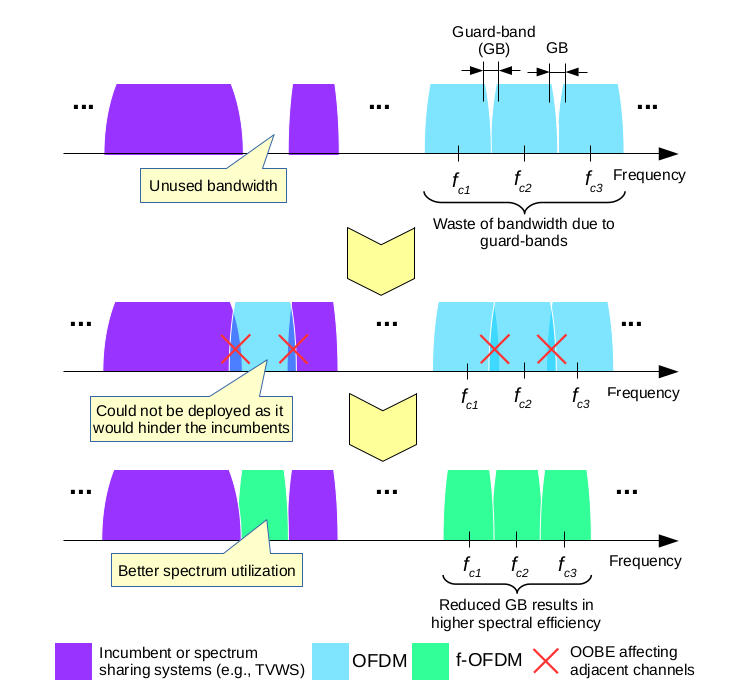
\includegraphics[width=0.6\textwidth]{Fig 1.png}
    \caption{Signals at adjacent frequencies.}
    \label{fig: 1}
\end{figure}
\end{frame}
\begin{frame}{Objective}
    \begin{itemize}
        \item The aim of this work is to show the results obtained by simulation comparing OFDM and f-OFDM techniques in Multiple Input Multiple Output systems(MIMO).
        \item It also evaluates the performance of various MIMO detectors.
        \begin{block}{Various MIMO detectors}
        \begin{itemize}
            \item Maximum Ratio Combining (MRC)
            \item Zero Forcing (ZF)
            \item Minimum Mean Squared Error(MMSE)
            \item Maximum Likelihood (ML)
            \item Sphere Decoding (SD)
        \end{itemize}
        \end{block}
        \item Particular attention is paid to SD as it's performance is similar to ML with reduced complexity.
    \end{itemize}
\end{frame}
\begin{frame}{System Model}
    \begin{itemize}
        \item The employed study model was MIMO for transmission and reception in two scenarios.
        \begin{enumerate}
            \item Each transmitted signal goes through OFDM modulation.
            \item Each transimtted signal goes through f-OFDM modulation.
        \end{enumerate}
        \item The model is based on transmission sets of four signals at 3 different frequencies($f_{c1},f_{c2},f_{c3})$ as shown in figure \ref{fig: 1}, in both scenarios as it is possible to evaluate the effect of filtering on OFDM signals.
        \item We consider K=4 single antenna devices continuously transmitting signals at each one of the three available frequencies and a Base Station equipped with M antennas receiving and demodulating these signals.
    \end{itemize}
\end{frame}
\begin{frame}{System Model(contd.)}
    \begin{itemize}
        \item Here, we create an OFDM symbol by applying a 128 point IFFT to the input signal, however only 72 subcarriers are used for transmission.(remaining is left for guard band).
        \item The subcarriers are placed at 15KHz apart, that implies 72 x 15 =1.08MHz of useful bandwith.
        \item This is equivalent to a 1.4 MHz LTE signal where 1.08 MHz is the useful bandwidth and the rest is for guard band.
    \end{itemize}
\end{frame}
\begin{frame}{System Model Equation}
    \begin{block}{}
    The received signals from K antennas at a BS which is equipped with M antennas can be modeled as
    \begin{equation}
        y= Hs+n
    \end{equation}
    where
    \begin{itemize}
        \item s is $K \times 1$ transmitted signal vector
        \item y is $M \times 1$ received signal vector
        \item H is $M \times K$ channel matrix
        \item n is $M \times 1$ Guassian noise vector
    \end{itemize}
    \end{block}
    \end{frame}
\begin{frame}{Hypothetical System Model}
  \begin{figure}[H]
    \centering
    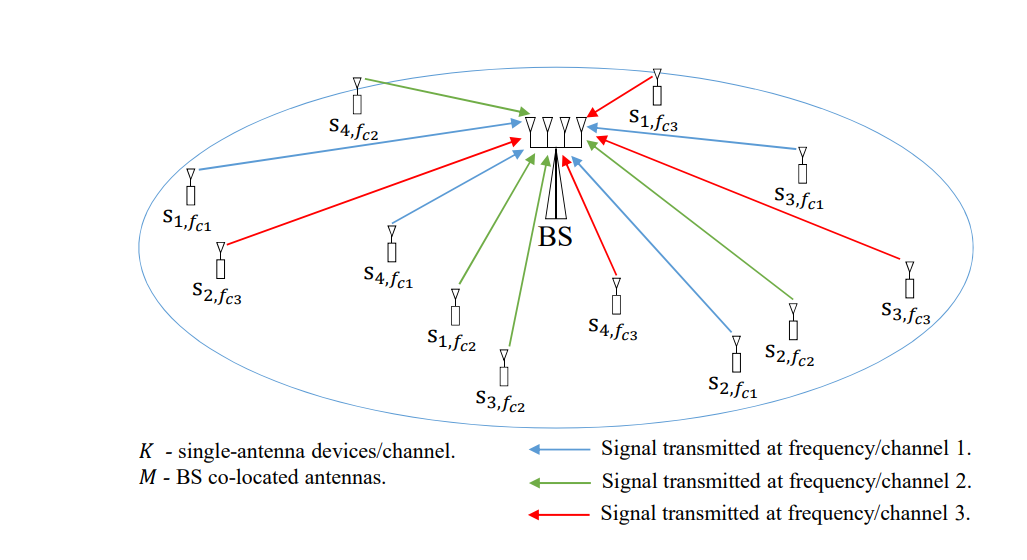
\includegraphics[width=0.8\textwidth]{fig 2.png}
    \caption{System model}
    \label{fig: 2}
\end{figure}
\end{frame}
\begin{frame}{Results and Discussion}{Extent of reduction in OOBE}
    \begin{itemize}
        \item We employ the system model depicted in figure \ref{fig: 2} and focus on the detection and performance of the signal at central frequency.
        \item  In figure \ref{fig: 3} we can see the power spectral density(PSD).
        \item We can see that the addition of FIR filter drastically reduces the OOBE.
        \item This reduction ranges from $-40 dBW/Hz$ to $-100 dBW/Hz$ , $-110 dBW/Hz$ ,$-120 dBW/Hz$ at a frequency of $0.4 \times fs$ (fs is sampling rate) with FIR filters of order 32,64,128 respectively.
        \end{itemize}
\end{frame}
\begin{frame}{Comparison}
\begin{figure}[H]
    \centering
    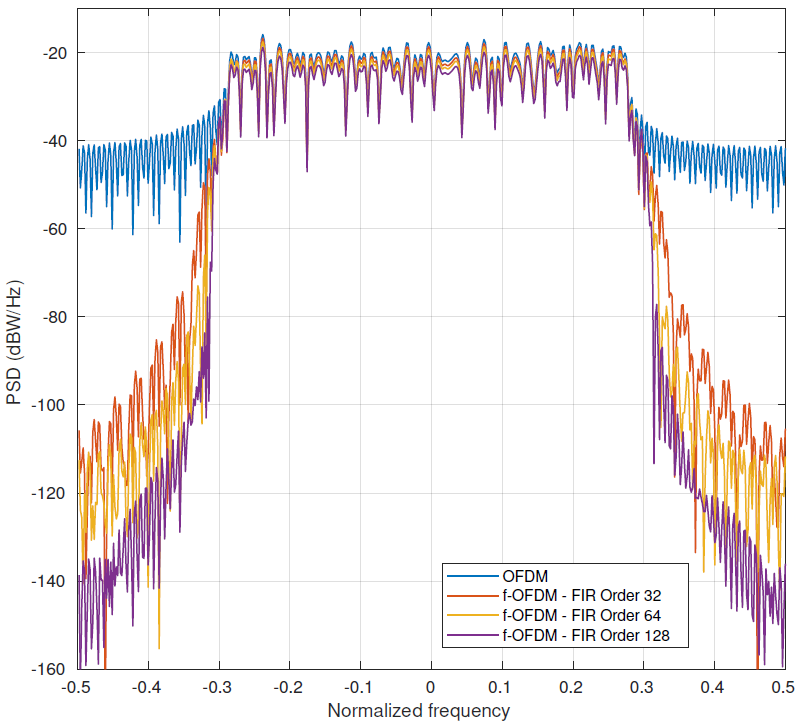
\includegraphics[width=0.6\textwidth]{fig 3.png}
    \caption{OFDM and f-OFDM PSD for filter orders 32, 64 and 128}
    \label{fig: 3}
\end{figure}
\end{frame}
\begin{frame}{Results and Discussion(Contd.)}{Showing Filter's energy lies within the CP}
\begin{itemize}
    \item Figure \ref{fig: 4} shows the base-band impulse response of the designed filter with bandwidth equal to $72 \times 15 KHz + 2 \times N_e$.
    \item We can see that the main energy of the filters is confined within the main lobe,which expands to $2.084\mu s$.
    \item Therefore, the filter's energy stays within the CP(cyclic prefix) length(for normal CP length is $4.7 \mu s$) and hence ISI(inter symbol interference) stays within tolerable levels.
\end{itemize}
\end{frame}
\begin{frame}{Impulse response of the designed filter}
\begin{figure}
    \centering
    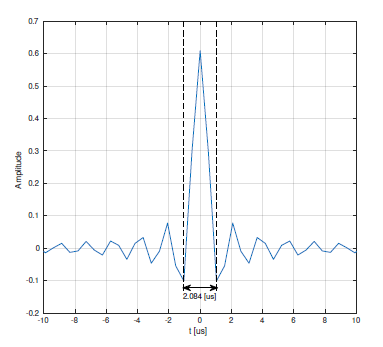
\includegraphics[width=0.6\textwidth]{fig 4.png}
    \caption{Impulse response of the designed filter for f-OFDM with bandwidth
equal to $72 \times 15 KHz + 2 \times N_e$.}
    \label{fig: 4}
\end{figure}
\end{frame}
\begin{frame}{Frequency responses of the designed filters for f-OFDM}
    \begin{figure}
        \centering
        \begin{subfigure}[b]{0.3\textwidth}
         \centering
         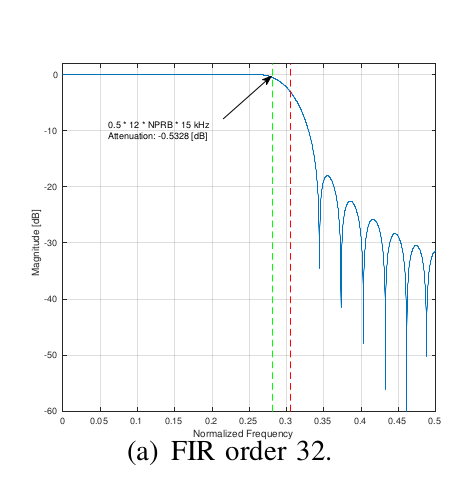
\includegraphics[width=\textwidth]{Fig 5(1).png}
         \caption{}
         \label{fig:5(1)}
        \end{subfigure}
        \hfill
        \begin{subfigure}[b]{0.3\textwidth}
         \centering
         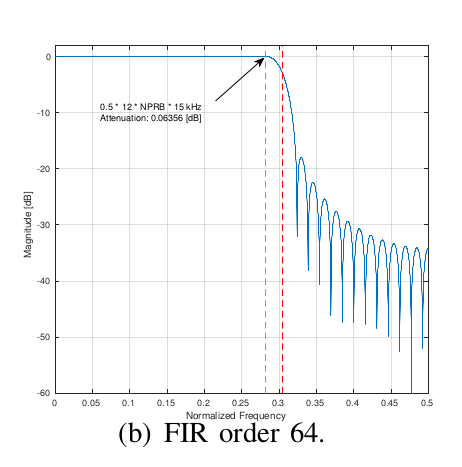
\includegraphics[width=\textwidth]{Fig 5(2).png}
         \caption{}
         \label{fig:5(2)}
        \end{subfigure}
        \hfill
        \begin{subfigure}[b]{0.3\textwidth}
         \centering
         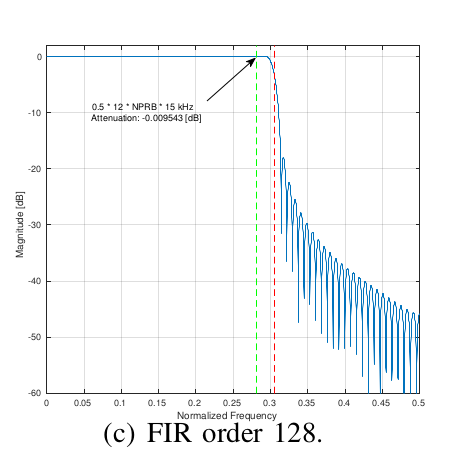
\includegraphics[width=\textwidth]{Fig 5(3).png}
         \caption{}
         \label{fig:5(3)}
        \end{subfigure}
        \caption{Frequency responses of the designed filters for f-OFDM having filter orders 32 (a), 64 (b), 128 (c).}
        \label{fig:5}
    \end{figure}
\end{frame}
\begin{frame}{Results and Discussion(Contd.)}{Attenuation and 3dB cutoff frequency}
\begin{itemize}
    \item The figure \ref{fig:5} shows the 3 dB cutoff frequency (red-dashed lines) of the filters, which, as designed, happens at half of the useful bandwidth plus
the excess bandwidth($N_e$).    
 \ie
 
    $108/2$ MHz +$3 \times 15$KHZ = $584$KHz.

  \item The 128 order filter shows a steeper transition,which results in lesser interference and hence a better frequency localization when compared with OFDM.
  \item As the filter order increases ,the subcarriers at the edges(green-dashed lines) of the symbol are less effected by attenuation.
\end{itemize}
\end{frame}
\begin{frame}{BER evaluations}
    \begin{figure}
        \centering
        \begin{subfigure}[b]{0.3\textwidth}
         \centering
         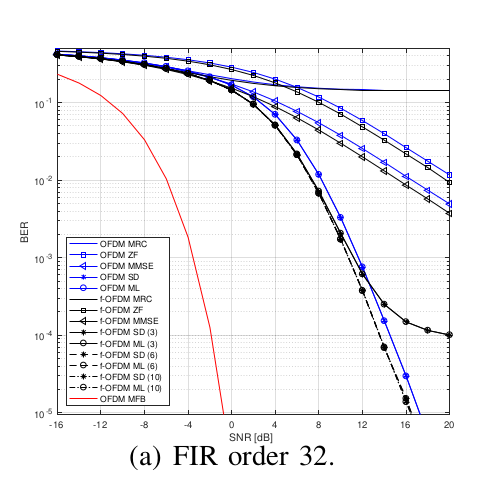
\includegraphics[width=\textwidth]{Fig 6(1).png}
         \caption{}
         \label{fig:6(1)}
        \end{subfigure}
        \hfill
        \begin{subfigure}[b]{0.3\textwidth}
         \centering
         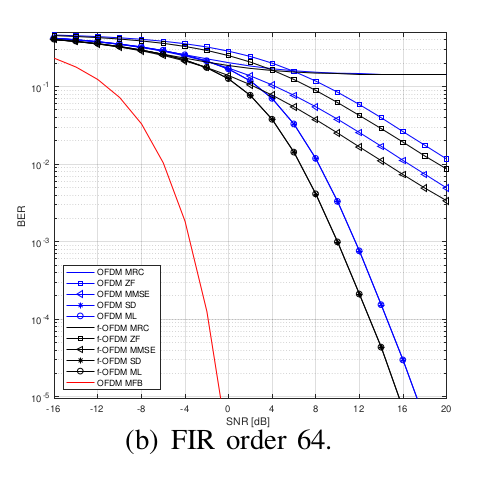
\includegraphics[width=\textwidth]{Fig 6(2).png}
         \caption{}
         \label{fig:6(2)}
        \end{subfigure}
        \hfill
        \begin{subfigure}[b]{0.3\textwidth}
         \centering
         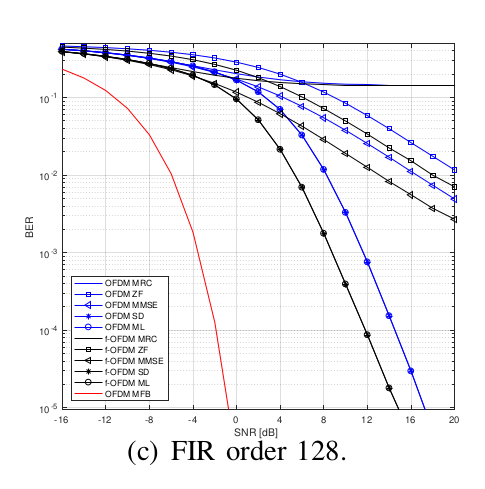
\includegraphics[width=\textwidth]{Fig 6(3).png}
         \caption{}
         \label{fig:6(3)}
        \end{subfigure}
        \caption{BER performance for MIMO OFDM versus MIMO f-OFDM detection with filter orders 32 (a), 64 (b), 128 (c)}
        \label{fig: 6}
    \end{figure}
\end{frame}
\begin{frame}{Results and Discussion(Contd.)}{Comparing BER and MIMO detector performances}
\begin{itemize}
    \item In the figure \ref{fig: 6}, we present the Bit Error Rate(BER) evaluation,which is taken as average over all subcarriers carrying data.
    \item For better comparison we also add the MFB(Matched Filter Bound) to the graph, which is also known as perfect interference-cancellation bound.
    \item It can be seen that the BER of f-OFDM is lower compared to OFDM and it further decreases with increasing filter order.
    \item Hence,we see that f-OFDM with SD and ML detectors approaches MFB faster as filter order increases.
    \item It is important to note that SD and ML show similar performance though SD has lesser complexity than ML. 
\end{itemize}
\end{frame}
\begin{frame}{Results and Discussion(Contd.)}{Disadvantage of f-OFDM and solution}
    \begin{itemize}
        \item It is also important to notice that for a filter order of 32 and $N_e$ = 3 the BER for SD and ML detectors reaches a BER floor of approximately $10^{-4}$ for SNR greater than 12 dB. 
        \item From there, f-OFDM behaves worse than the OFDM with SD and ML detection.
        \item This is due to, the subcarries at the edges are heavily affected by filter's poor performance at the edges(\ie attenuation becomes noticeable).
        \item In order to validate our assumption, we also show the BER evaluations for excess bandwidth,$N_e$,of 3 and 10 subcarriers.This makes the edges flatter and therefore we do not see any unusual curve.
    \end{itemize}
\end{frame}
\begin{frame}{Results and Discussion(Contd.)}{Effect of number of antennas at Base Station}
    \begin{itemize}
        \item In figure \ref{fig: 7} we see the BER performance of the detectors approaches MFB with increase in the number of antennas at the Base Station(BS).
        \item These results clearly prove that the interference caused by users transmitting at closely separated adjacent channels can be reduced by having a BS equipped with a large number of antennas.
    \end{itemize}
\end{frame}
\begin{frame}{Effect of number of Base Station antennas }
    \begin{figure}
        \centering
        \begin{subfigure}[b]{0.23\textwidth}
         \centering
         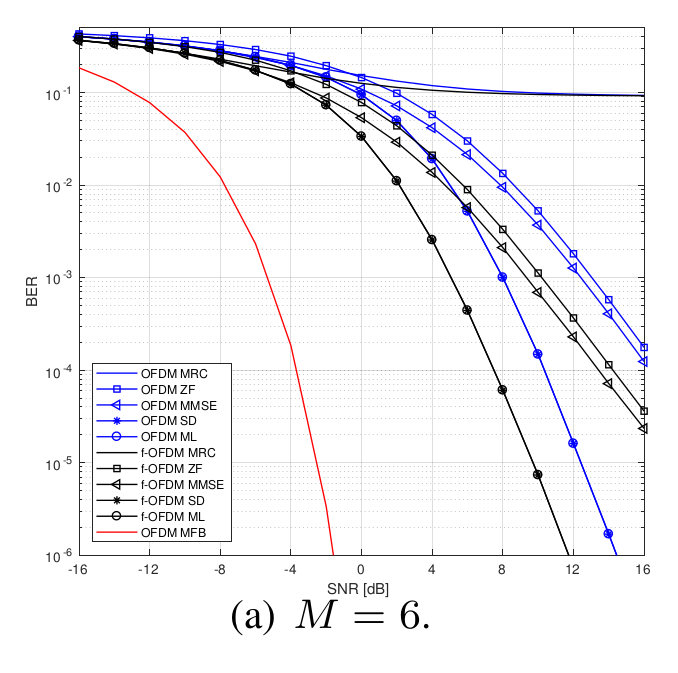
\includegraphics[width=\textwidth]{Fig 7(1).png}
         \caption{}
         \label{fig:7(1)}
        \end{subfigure}
        \hfill
        \begin{subfigure}[b]{0.23\textwidth}
         \centering
         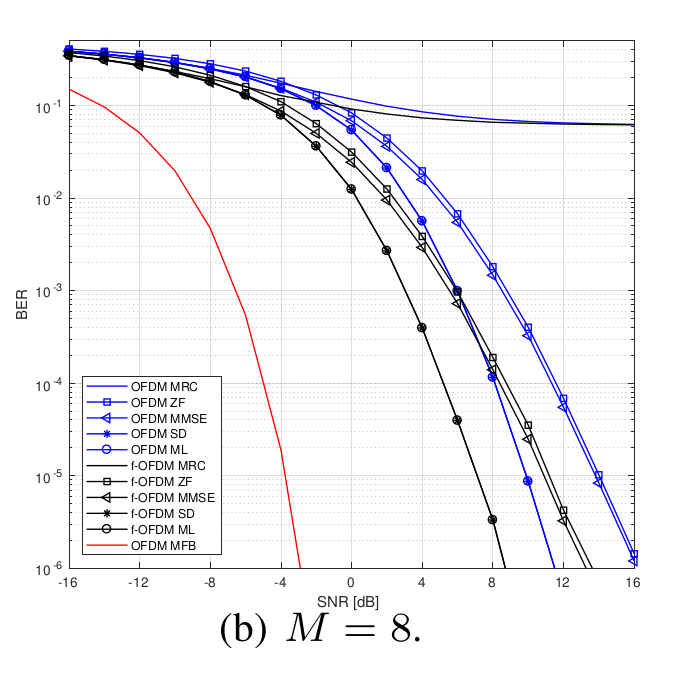
\includegraphics[width=\textwidth]{Fig 7(2).png}
         \caption{}
         \label{fig:7(2)}
        \end{subfigure}
        \hfill
        \centering
        \begin{subfigure}[b]{0.23\textwidth}
         \centering
         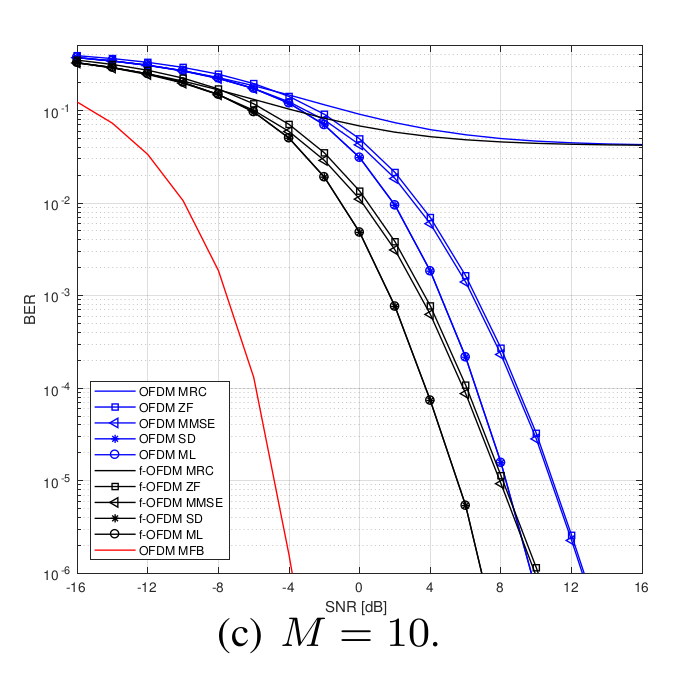
\includegraphics[width=\textwidth]{Fig 7(3).png}
         \caption{}
         \label{fig:7(3)}
        \end{subfigure}
        \hfill
        \centering
        \begin{subfigure}[b]{0.23\textwidth}
         \centering
         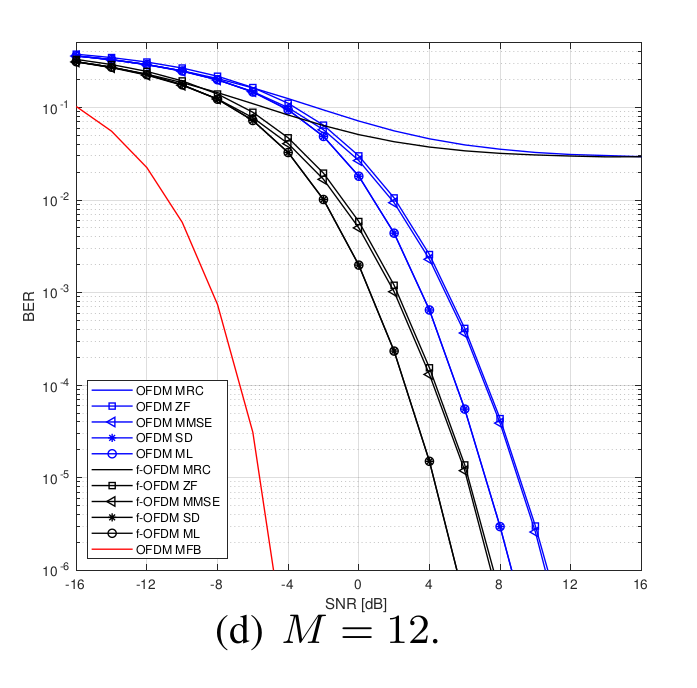
\includegraphics[width=\textwidth]{Fig 7(4).png}
         \caption{}
         \label{fig:7(4)}
        \end{subfigure}
        \caption{BER performance for MIMO OFDM versus MIMO f-OFDM detection,filter order 128,number of antennas,M}
        \label{fig: 7}
    \end{figure}
\end{frame}
\begin{frame}{Results and Discussion(Contd.)}{Drawback of f-OFDM}
    \begin{itemize}
    \item With increase in PAPR(Peak to average power ratio), the amplification becomes a problem.
    \item In figure \ref{fig: 8},we assess the PAPR by a single carrier,in both OFDM and f-OFDM. Here , we measure the CCDF(Complementary Cumulative Distribution Frequency) for each of the modulations.
    \item We observe that the probability of the power of the OFDM and f-OFDM modulated signals being more than 3 dB above its average power level is higher than for a QAM modulated signal.
    \item Although f-OFDM reduces OOBE,it presents as a drawback, a PAPR that is higher than that for OFDM which still increases with increase in filter order.
    \end{itemize}
\end{frame}
\begin{frame}{CCDF}
    \begin{figure}
        \centering
        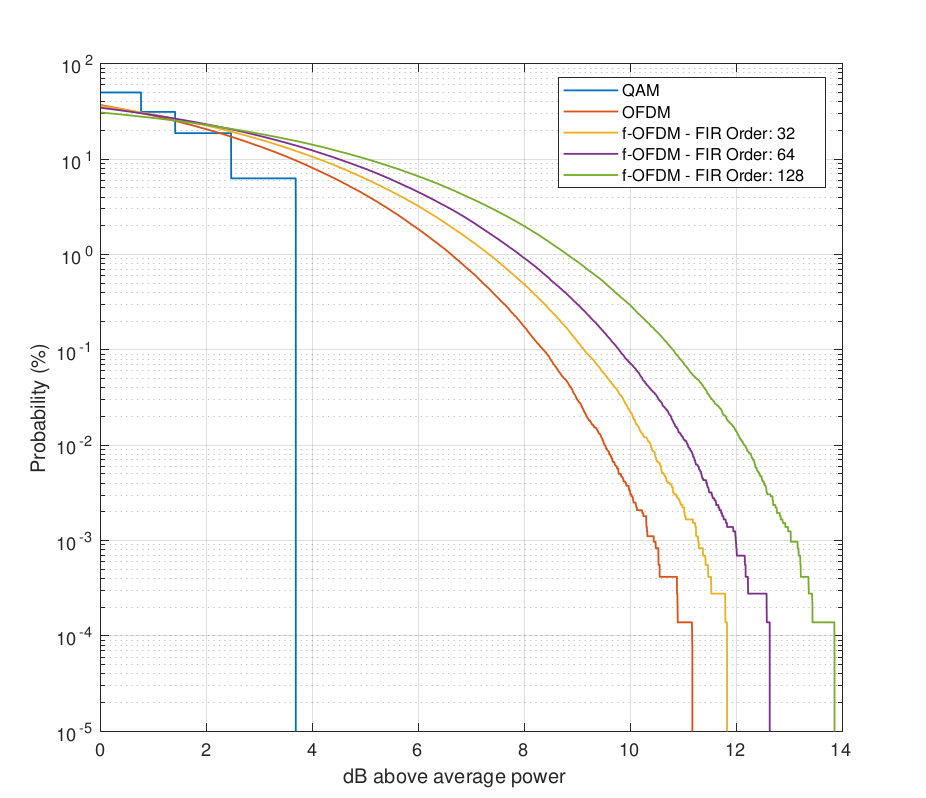
\includegraphics[width=0.6\textwidth]{Fig 8.png}
        \caption{CCDF comparison of single-carrier and OFDM/f-OFDM modulation schemes.}
          \label{fig: 8}
    \end{figure}
\end{frame}
\begin{frame}{Conclusion}
\begin{itemize}
    \item In this paper, we assessed the interference among adjacent signals in a MIMO system with OFDM and f-OFDM.
    \item The MIMO system performance was analysed by BER evaluations using detectors.
    \item Our analysis conclude that f-OFDM equipped systems perform better when power amplification factor is not an issue.Given this condition, f-OFDM acts as an excellent candidate for future generations of wireless communications.
    \item Therefore, f-OFDM systems allow closer frequency coexistence of devices, which increases the spectral efficiency, as the distance among adjacent channels can be decreased.
\end{itemize}
\end{frame}
\end{document}

